% Options for packages loaded elsewhere
\PassOptionsToPackage{unicode}{hyperref}
\PassOptionsToPackage{hyphens}{url}
%
\documentclass[
  12pt,
]{article}
\usepackage{lmodern}
\usepackage{setspace}
\usepackage{amssymb,amsmath}
\usepackage{ifxetex,ifluatex}
\ifnum 0\ifxetex 1\fi\ifluatex 1\fi=0 % if pdftex
  \usepackage[T1]{fontenc}
  \usepackage[utf8]{inputenc}
  \usepackage{textcomp} % provide euro and other symbols
\else % if luatex or xetex
  \usepackage{unicode-math}
  \defaultfontfeatures{Scale=MatchLowercase}
  \defaultfontfeatures[\rmfamily]{Ligatures=TeX,Scale=1}
\fi
% Use upquote if available, for straight quotes in verbatim environments
\IfFileExists{upquote.sty}{\usepackage{upquote}}{}
\IfFileExists{microtype.sty}{% use microtype if available
  \usepackage[]{microtype}
  \UseMicrotypeSet[protrusion]{basicmath} % disable protrusion for tt fonts
}{}
\makeatletter
\@ifundefined{KOMAClassName}{% if non-KOMA class
  \IfFileExists{parskip.sty}{%
    \usepackage{parskip}
  }{% else
    \setlength{\parindent}{0pt}
    \setlength{\parskip}{6pt plus 2pt minus 1pt}}
}{% if KOMA class
  \KOMAoptions{parskip=half}}
\makeatother
\usepackage{xcolor}
\IfFileExists{xurl.sty}{\usepackage{xurl}}{} % add URL line breaks if available
\IfFileExists{bookmark.sty}{\usepackage{bookmark}}{\usepackage{hyperref}}
\hypersetup{
  pdftitle={Núcleo de Estudos em Representação e Democracia},
  hidelinks,
  pdfcreator={LaTeX via pandoc}}
\urlstyle{same} % disable monospaced font for URLs
\usepackage[left=3cm,right=3cm,top=2cm,bottom=2cm]{geometry}
\usepackage{graphicx,grffile}
\makeatletter
\def\maxwidth{\ifdim\Gin@nat@width>\linewidth\linewidth\else\Gin@nat@width\fi}
\def\maxheight{\ifdim\Gin@nat@height>\textheight\textheight\else\Gin@nat@height\fi}
\makeatother
% Scale images if necessary, so that they will not overflow the page
% margins by default, and it is still possible to overwrite the defaults
% using explicit options in \includegraphics[width, height, ...]{}
\setkeys{Gin}{width=\maxwidth,height=\maxheight,keepaspectratio}
% Set default figure placement to htbp
\makeatletter
\def\fps@figure{htbp}
\makeatother
\setlength{\emergencystretch}{3em} % prevent overfull lines
\providecommand{\tightlist}{%
  \setlength{\itemsep}{0pt}\setlength{\parskip}{0pt}}
\setcounter{secnumdepth}{-\maxdimen} % remove section numbering

\title{Núcleo de Estudos em Representação e Democracia}
\usepackage{etoolbox}
\makeatletter
\providecommand{\subtitle}[1]{% add subtitle to \maketitle
  \apptocmd{\@title}{\par {\large #1 \par}}{}{}
}
\makeatother
\subtitle{NERD}
\author{}
\date{\vspace{-2.5em}}

\begin{document}
\maketitle

\setstretch{1.5}
\hypertarget{apresentauxe7uxe3o}{%
\subsection{1. Apresentação}\label{apresentauxe7uxe3o}}

\hfill\break O Núcleo de Estudos em Representação e Democracia -- NERD,
tem por objetivo promover pesquisas sobre a evolução política e
eleitoral nos níveis subnacionais, principalmente no nível municipal,
assim como a relação da mesma com o desenvolvimento.

O grupo de pesquisa aborda a interseção entre três grandes dimensões da
análise de sistemas políticos democráticos: governos, comportamento
eleitoral e partidos políticos. A partir dos estudos sobre comportamento
dos eleitores pretende-se integrar os achados empíricos às teorias sobre
estratégias dos partidos políticos nas administrações públicas
subnacionais, assim como interagir com análises sobre reeleição de
prefeitos, análises que abordam ideologia partidária e gastos públicos
no Brasil.

O NERD tem o objetivo de abranger estudos sobre política nacional
visando estudos e análises comparadas. As atividades do NERD procuram
atender a demanda de informações e análises no Brasil, tendo em conta
que existe uma considerável escassez de informações empíricas sobre as
características, funcionamento e desempenho das instituições políticas
no nível municipal, assim como da interação da dimensão política com o
desenvolvimento socioeconômico.

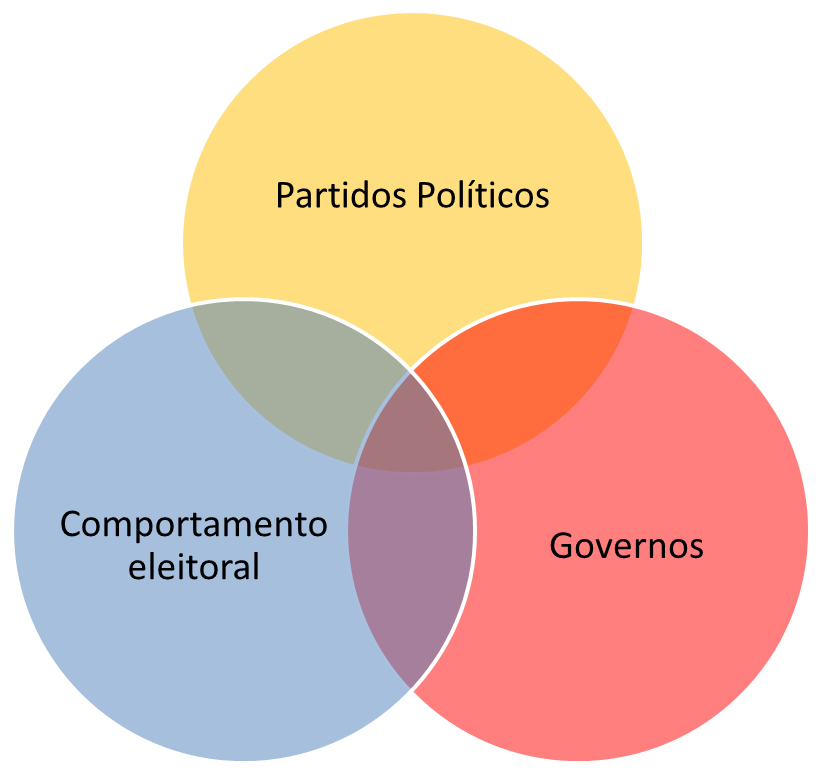
\includegraphics{nerd_diagrama_venn.png}

O núcleo teve início da suas atividades com o projeto de pesquisa
``Competição Eleitoral nos Municípios Brasileiros'', em 2011, deu
sequencia com o projeto CNPq ``Poder Local, Partidos políticos e
eleições municipais no Brasil pós 1988'', e atualmente é financiado pela
FAPERJ com projeto ``Petro rendas e política local: competição eleitoral
e políticas públicas em municípios produtores de petróleo''.

\begin{itemize}
\tightlist
\item
  Projeto FAPERJ E-26/111-677/2011.``Competição Eleitoral nos Municípios
  Brasileiros''
\item
  Projeto CNPq: ``Poder local, Partidos políticos e eleições municipais
  no Brasil pós 1988''.
\item
  Projeto FAPERJ APQ3 E-26/112.214/2013. ``Financiamento de campanhas
  eleitorais no Brasil''.
\item
  Projeto FAPERJ - E-26/210-545/2019. ``Petro rendas e política local:
  competição eleitoral e políticas públicas em municípios produtores de
  petróleo''.
\end{itemize}

\hypertarget{justificativa-melhorar-esta-justificativa}{%
\subsection{2. Justificativa (melhorar esta
justificativa)}\label{justificativa-melhorar-esta-justificativa}}

\hfill\break  No Brasil existe uma considerável escassez de informações
empíricas sobre o desempenho e funcionamento das instituições políticas
municipais e das interações com o desenvolvimento socioeconômico. O
Núcleo de Estudos em Representação e Democracia -- NERD, procura
contribuir para solucionar esse déficit. A maioria dos trabalhos que
abordam o tema da política municipal, analisa as capitais estaduais ou
municípios que introduziram novas formas de participação, como o
orçamento participativo e os conselhos municipais.

A Constituição de 1988 se orienta claramente por um princípio
descentralizador e municipalista. No Capítulo IV (``Dos Municípios''),
artigo 29 se estabelece que ``o município reger-se-á por lei orgânica,
votada em dois turnos, com interstício mínimo de dez dias, e aprovada
por dois terços da Câmara Municipal (\ldots)''. Já no artigo 30 do mesmo
capítulo se estabelecem as competências dos municípios, em que se
destacam as áreas de educação pré-escolar, ensino fundamental, saúde e
saneamento, podendo ser solicitado para o cumprimento dessas funções, a
cooperação técnica e financeira do Estado e da União. Incumbe também aos
governos municipais instituir e arrecadar os tributos correspondentes a
suas competências, assim como a alocação das receitas.

Junto com o incremento da autonomia municipal e de suas atribuições nas
áreas mencionadas, a Constituição também valorizou os legislativos
municipais, outorgando-lhes a possibilidade de introduzir emendas ao
orçamento municipal, reforçando o poder político das Câmaras de
Vereadores. Além dessa nova potestade, a relevância desses órgãos radica
não somente na visibilidade dos temas sobre os que devem legislar muito
próximos da vida cotidiana dos cidadãos, mas também, no vínculo direto
de seus membros com as bases eleitorais. Porém, vários trabalhos têm
destacado a hipertrofia dos Executivos nos municípios pequenos e médios,
em relação aos Legislativos e Judiciários (Abrucio, 1994; Nunes, 1991).

Concomitantemente ao aumento das responsabilidades e atribuições dos
municípios, houve também, a partir da aprovação da nova Constituição, um
aumento das fontes tributárias e um repasse automático de receitas por
parte dos Estados e do Governo Federal. Com efeito, as principais
consequências da reforma constitucional foram um aumento substancial do
poder tributário dos governos subnacionais nas suas respectivas
jurisdições e um incremento das transferências da União para Estados e
municípios (Abrucio e Couto, 1996; Giambiagi, 1991).

Os dados censitários a partir de 1991 indicaram um crescimento
populacional mais acelerado dos municípios de pequeno, médio e grande
porte. Ressalta-se que em alguns municípios de grande porte tal
perspectiva se manifestava com um ritmo de crescimento populacional
superior ao das Regiões Metropolitanas na década de 1970. Nestes termos,
Baeninger (1999: p.538), aponta para o fato de que ``os municípios
não-metropolitanos registraram um incremento relativo de 22\%, no
período 1970-1980, e de 6,7\% no de 1991-1996''. Assim, pode-se perceber
que o processo de interiorização que já vinha ocorrendo no Brasil em
décadas anteriores, continuou sendo observado, agudizando-se a partir
dos anos 2000.

Com base nestas considerações mais gerais propõe-se um núcleo de
pesquisa focalizado nas questões relativas à política e ao
desenvolvimento socioeconômico. As atividades do núcleo podem ser
agrupadas em dois grandes eixos analíticos. O primeiro refere-se ao
funcionamento das instituições políticas (eleições, administração
pública, comportamento parlamentar e relação executivo-legislativo). O
segundo eixo concerne ao desenvolvimento socioeconômico (atividades
produtivas, estrutura social, mercado de trabalho e perfil social dos
municípios). É objetivo do NERD, nos seus projetos de pesquisa e nas
suas atividades em geral, analisar as possíveis relações entre ambos
eixos temáticos. Inclui-se nesta proposta o intuito de contribuir com
produção de informação e conhecimento científico relevante sobre o
desenvolvimento político, econômico e social dos municípios brasileiros,
assim como estudos que abordem o desempenho político institucional de
outras regiões e municípios do país, possibilitando ainda a realização
de análises comparadas, outra dos objetivos do NERD.

\hypertarget{objetivos}{%
\subsection{3. Objetivos}\label{objetivos}}

\hfill\break  Como foi definido, o NERD, tem por objetivo promover
pesquisas sobre a evolução política e eleitoral no nível municipal,
assim como a relação da mesma com o desenvolvimento. O NERD tem o
objetivo de abranger estudos sobre política em todo o país, visando
estudos e análises comparadas.

Os objetivos específicos do núcleo a destacar são:

\begin{itemize}
\item
  Difusão dos resultados das pesquisas para o âmbito acadêmico e
  extra-acadêmico (encontros, seminários, mini-cursos, etc.).
\item
  Promover a participação de alunos de graduação (iniciação científica)
  e pós-graduação nas atividades do núcleo.
\item
  Organizar e compartilhar bases de dados destinados a subsidiar
  pesquisas acadêmicas e a demandas de instituições públicas e privadas,
  formadores de opinião e público em geral.
\item
  Participar em editais de financiamento de pesquisas e atividades de
  extensão.
\end{itemize}

\hypertarget{membros}{%
\subsection{4. Membros}\label{membros}}

\href{http://lattes.cnpq.br/4676437210734787}{Vitor de Moraes Peixoto}
\hfill\break \textbf{Coordenador} \hfill\break Professor Associado
\hfill\break Universidade Estadual do Norte Fluminense Darcy Ribeiro
\hfill\break Centro de Ciências do Homem \hfill\break Laboratório de
Estudos da Sociedade Civil e do Estado \hfill\break E-mail:
\href{mailto:moraespeixoto@gmail.com}{\nolinkurl{moraespeixoto@gmail.com}}

\href{http://lattes.cnpq.br/7250750885312461}{Ralph André Crespo}
\hfill\break Doutorando do Programa de Pós-Graduação em Sociologia
Politica \hfill\break Universidade Estadual do Norte Fluminense Darcy
Ribeiro \hfill\break Laboratório de Estudos do Estado e da Sociedade
Civil \hfill\break E-mail:
\href{mailto:pr.ralph@yahoo.com.br}{\nolinkurl{pr.ralph@yahoo.com.br}}
\hfill\break

\href{http://lattes.cnpq.br/1477388811747167}{Jheniffer Vieira de
Almeida} \hfill\break Doutoranda do Programa de Pós-Graduação em
Sociologia Politica \hfill\break Universidade Estadual do Norte
Fluminense Darcy Ribeiro \hfill\break Laboratório de Estudos do Estado e
da Sociedade Civil \hfill\break E-mail:
\href{mailto:jheniffer.vi@gmail.com}{\nolinkurl{jheniffer.vi@gmail.com}}
\hfill\break

\href{http://lattes.cnpq.br/9433034841064768}{Raphael de Mello Veloso}
\hfill\break Doutorando do Programa de Pós-Graduação em Sociologia
Politica \hfill\break Universidade Estadual do Norte Fluminense Darcy
Ribeiro \hfill\break Laboratório de Estudos do Estado e da Sociedade
Civil \hfill\break E-mail:
\href{mailto:raphamv@gmail.com}{\nolinkurl{raphamv@gmail.com}}

\href{http://lattes.cnpq.br/1675744772217864}{Gisele Braga Bastos}
\hfill\break Doutoranda do Programa de Pós-Graduação em Sociologia
Politica \hfill\break Universidade Estadual do Norte Fluminense Darcy
Ribeiro \hfill\break Laboratório de Estudos do Estado e da Sociedade
Civil \hfill\break E-mail:
\href{mailto:gibragabastos@gmail.com}{\nolinkurl{gibragabastos@gmail.com}}
\hfill\break

\href{http://lattes.cnpq.br/6717255818088404}{Jessica Matheus de Souza}
\hfill\break Doutoranda do Programa de Pós-Graduação em Sociologia
Politica \hfill\break Universidade Estadual do Norte Fluminense Darcy
Ribeiro \hfill\break Laboratório de Estudos do Estado e da Sociedade
Civil \hfill\break E-mail:
\href{mailto:jessicamatheus@outlook.com}{\nolinkurl{jessicamatheus@outlook.com}}
\hfill\break

\href{http://lattes.cnpq.br/8178088513307546}{Wallace da Silva Mello}
\hfill\break Doutorando do Programa de Pós-Graduação em Sociologia
Politica \hfill\break Universidade Estadual do Norte Fluminense Darcy
Ribeiro \hfill\break Laboratório de Estudos do Estado e da Sociedade
Civil \hfill\break E-mail:
\href{mailto:wallace_sm89@hotmail.com}{\nolinkurl{wallace\_sm89@hotmail.com}}
\hfill\break

\href{http://lattes.cnpq.br/5038496684551538}{Thiago Pimentel Soares}
\hfill\break Mestrando do Programa de Pós-Graduação em Sociologia
Politica \hfill\break Universidade Estadual do Norte Fluminense Darcy
Ribeiro \hfill\break Laboratório de Estudos do Estado e da Sociedade
Civil \hfill\break E-mail:
\href{mailto:tpsoares@hotmail.com}{\nolinkurl{tpsoares@hotmail.com}}
\hfill\break

\href{http://lattes.cnpq.br/6781198318316057}{Rafael Soares Salles}
\hfill\break Mestrando do Programa de Pós-Graduação em Sociologia
Politica \hfill\break Universidade Estadual do Norte Fluminense Darcy
Ribeiro \hfill\break Laboratório de Estudos do Estado e da Sociedade
Civil \hfill\break  E-mail:
\href{mailto:rafael.salles@outlook.com}{\nolinkurl{rafael.salles@outlook.com}}
\hfill\break

\href{http://lattes.cnpq.br/8424422005329610}{Larissa Martins Marques}
\hfill\break Graduanda do Curso de Administração Pública \hfill\break
Universidade Estadual do Norte Fluminense Darcy Ribeiro \hfill\break
Laboratório de Estudos do Estado e da Sociedade Civil \hfill\break
E-mail:
\href{mailto:larissamarques@pq.uenf.br}{\nolinkurl{larissamarques@pq.uenf.br}}
\hfill\break

\href{http://lattes.cnpq.br/6781198318316057}{Matheus Virginio Harduim
Machado} \hfill\break Graduando do Curso de Ciências Sociais
\hfill\break niversidade Estadual do Norte Fluminense Darcy Ribeiro
\hfill\break Laboratório de Estudos do Estado e da Sociedade Civil
\hfill\break E-mail:
\href{mailto:mattharduim@gmail.com}{\nolinkurl{mattharduim@gmail.com}}
\hfill\break

\href{http://lattes.cnpq.br/7181203038300743}{Fernanda da Silva Souza}
\hfill\break Graduanda do Curso de Ciências Sociais \hfill\break
niversidade Estadual do Norte Fluminense Darcy Ribeiro \hfill\break
Laboratório de Estudos do Estado e da Sociedade Civil \hfill\break
E-mail:
\href{mailto:fer.souzaa1@outlook.com}{\nolinkurl{fer.souzaa1@outlook.com}}
\hfill\break

\href{http://lattes.cnpq.br/6943283489647623}{Lara Bernardo de Oliveira}
\hfill\break Graduanda do Curso de Ciências Sociais \hfill\break 
niversidade Estadual do Norte Fluminense Darcy Ribeiro \hfill\break
Laboratório de Estudos do Estado e da Sociedade Civil \hfill\break
E-mail:
\href{mailto:lalabernardo1904@gmail.com}{\nolinkurl{lalabernardo1904@gmail.com}}
\hfill\break

\href{}{Paula Regis} \hfill\break Graduanda do Curso de Administração
Pública \hfill\break Universidade Estadual do Norte Fluminense Darcy
Ribeiro \hfill\break Laboratório de Estudos do Estado e da Sociedade
Civil \hfill\break E-mail:
\href{mailto:regispaularegis@gmail.com}{\nolinkurl{regispaularegis@gmail.com}}
\hfill\break

\hfill\break \hfill\break Falta inserir os pós doutorandos.
\hfill\break \hfill\break

\hypertarget{localizauxe7uxe3o}{%
\subsection{5. Localização}\label{localizauxe7uxe3o}}

\hfill\break \hfill\break Universidade Estadual do Norte Fluminense
Darcy Ribeiro \hfill\break Centro de Ciências do Homem -- CCH -- Sala
108 - B \hfill\break Av. Alberto Lamego, 2000 - Parque Califórnia
\hfill\break Campos dos Goytacazes - RJ \hfill\break CEP: 28013-602
\hfill\break Tel: 22 27397040 \hfill\break

\end{document}
